\section{CLABEL Add Labels To Contour Plot}

\subsection{Usage}

The \verb|clabel| function adds labels to a contour plot
Generate contour labels for a contour plot.  The syntax
for its use is either:
\begin{verbatim}
   handles = clabel(contourhandle,property,value,property,value,...)
\end{verbatim}
which labels all of the contours in the plot, or
\begin{verbatim}
   handles = clabel(contourhandle,vals,property,value,property,value,...)
\end{verbatim}
which only labels those contours indicated by the vector \verb|vals|.
The \verb|contourhandle| must be the handle to a contour plot object.
The remaining property/value pairs are passed to the \verb|text| function
to control the parameters of the generated text labels.  See the 
\verb|text properties| for the details on what can be used in those labels.
\subsection{Example}

\begin{verbatim}
--> [x,y] = meshgrid(linspace(-1,1,50));
--> z = x.*exp(-(x.^2+y.^2));
--> h = contour(z);
--> clabel(h,'backgroundcolor',[1,1,.6],'edgecolor',[.7,.7,.7]);
\end{verbatim}
which results in


\centerline{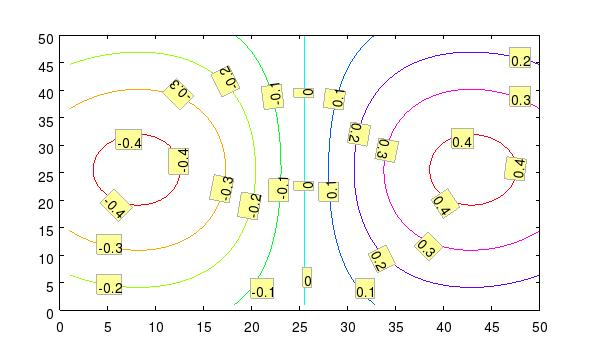
\includegraphics[width=8cm]{clabel1}}

Alternately, we can just label a subset of the contours
\begin{verbatim}
--> h = contour(z);
--> clabel(h,[-.2,0,.3]);
\end{verbatim}
which results in


\centerline{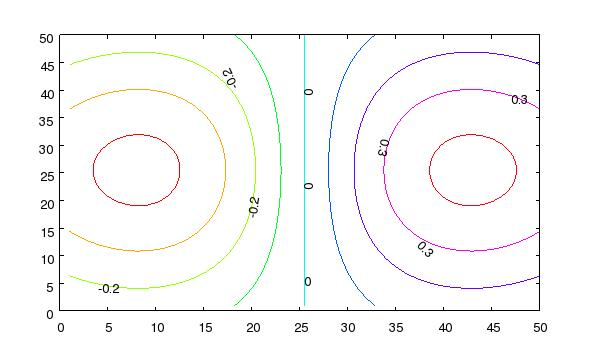
\includegraphics[width=8cm]{clabel2}}

